\documentclass[english,a4paper]{ifimaster}
\usepackage[utf8]{inputenc}
\usepackage[T1]{fontenc,url}
\urlstyle{sf}
\usepackage{babel,textcomp,csquotes,ifimasterforside,varioref,graphicx}
\usepackage[backend=bibtex,style=numeric-comp]{biblatex}
\usepackage{wrapfig}
\usepackage{subcaption}
\usepackage{float}
\usepackage{fancyvrb}

\DefineVerbatimEnvironment{code}{Verbatim}{fontsize=\small}

\newcommand{\enwikicatlink}{\texttt{enwiki-latest-categorylinks.sql.gz} }
\newcommand{\enwikipage}{\texttt{enwiki-latest-page.sql.gz} }
\newcommand{\enwikicategory}{\texttt{enwiki-latest-category.sql.gz} }
\newcommand{\catlinkprogram}{\texttt{Split\_catlink.py}}
\newcommand{\catgraphbuilderprogram}{\texttt{Categorygraph\_builder.py}}

\title{Content Categorization for Contextual Advertising Using Wikipedia}
\author{Ingrid Grønlie Guren}

\bibliography{mybib}

\begin{document}
\ififorside{}
\frontmatter{}
\maketitle{}


% url for footnotes
\urldef\nowikidump\url{http://dumps.wikimedia.org/nowiki/latest/}
\urldef\categorytree\url{http://no.wikipedia.org/w/index.php?title=Spesial%3AKategoritre&target=Astrid+Lindgren&mode=categories&namespaces= }.
\urldef\olejohandahleng\url{http://en.wikipedia.org/wiki/Ole-Johan_Dahl}
%\urldef\iababout\url{http://www.iab.net/about_the_iab}

%%---------------------------------------------------------------------------%%

\chapter*{Abstract}
Automatic categorization of content is an important %piece of 
functionality in online advertising and automated content recommendations, both for ensuring contextual relevancy of placements and for building up behavioral profiles for users that consume the content. Within the advertising domain, the taxonomy tree that content is classified into is defined with some commercial application in mind and needs to somehow reflect the advertising platform’s ad inventory. The nature of the ad inventory and the language of the content might vary across brokers (i.e., the operator of the advertising platform), so it is of interest to develop a system that can easily bootstrap the development of a well-working classifier. Brokers are often not very technical and by experience will have severe problems developing training sets or otherwise contribute to the process, so any required involvement from their side has to be relatively simple. Furthermore, it is a practical requirement that the classifier can “explain” its classification to the broker in some way, and that the broker can have a simple way to manually override or influence the classification of known problem cases.

We explore the use of Wikipedia to develop a simple dictionary-based classifier. A dictionary-based classifier offers a simple way to “explain” the classification, and allows the classification vocabulary (i.e., the dictionary entries) to be easily edited. Wikipedia exists in a large number of languages, has a large number of article keywords covering most domains, and explicitly associates article names with categories. We describe a set of tools that automate the process of building up dictionaries that map Wikipedia keywords (or cleansed versions thereof) into Wikipedia categories (or modified versions thereof). Creating a mapping that maps Wikipedia categories into the broker’s custom taxonomy tree is a relatively straightforward task that brokers (or people working on their behalf) are assumed capable of. We will here use predefined a taxonomy, the one provided by IAB, as a working example of such a custom taxonomy tree.

Given such a classifier, we describe an experiment using a real advertising platform to validate its use in real life using real data. We also provide a brief overview of related work described in the literature.

\tableofcontents{}
\listoffigures{}
\listoftables{}

\chapter*{Acknowledgements}
This study has been a project for Xcense (\url{http://www.cxense.com}) and the Department of Informatics at the University of Oslo, and was started in the Winter semester  2014 and finished ** 2015. 

I would like to express my gratitude to my supervisor Aleksander Øhrn for 

Finally I would like to thank my family and study friends for all help, comments and discussions, and most importantly for supporting me every day.  
\mainmatter{}

\part{Introduction}
\chapter{The project}

\[ Put introduction here. \]
\part{Background}
\chapter{About content analysis}
Content analysis is the task of analysing and understanding collections of texts, in other words finding out what a text "is about". The task can be performed by both humans and computers, where both of the approaches have their advantages and disadvantages.

The concept of manual content analysis is easy, where the task is split into first reading and understanding the text, and then summarizing the content of the text and/or categorize it into suitable categories. For instance an article about Astrid Lindgren (the famous Swedish children books' author) would probably be summarized as an article about a famous Swedish children's author and might be categorized under the category "Swedish children's writers" if this category is present.  
%as an article about authors of children books and Swedish people. 
There are two main disadvantages of human content analysis. The first disadvantage is that the task is time consuming, i.e. it takes time to read and understand an article, and the second is that it requires resources that might be expensive, for instance experts needed for understanding the content of an article if the article is about something beyond common knowledge.

%because some articles needs experts for understanding the content. 

%first has to be read and understood and then we could summarize the content of the text or categorize it under relevant topics.
Computer content analysis is based on a different approach; instead of reading and understanding the text, the computer looks for words or phrases that are known and uses these to find the category of the text. There are some issues with computer content analysis that are important to handle. The first is that the computer cannot define its own categories, but needs a predefined set of possible categories. It is a lot easier to ask the computer "Is the article about a children's author?" than to let the computer find this possibility itself. The other issue is to decide what words are important and useful for deciding the categories of a text. 

%The computer content analysis is an automatic categorization process, where we want to find words that help us define the categories of the text. 
The first issue can be solved by defining a set of categories that we want to categorize text into. There are some requirements that need to be met for our set; the set has to be so large that all relevant texts can be placed under at least one category, and it has to be so general that similar texts have a high probability of being categorized together. The category set should also contain a special category \textit{unknown} for texts where no category is found. Another requirement for the category set is that the it has to be so well-defined and specific that it conserves as much information as possible about the categorized text. The solution to the problem should also be able to change the pre-defined category set to another pre-defined set depending on the texts that are being categorized and the context of the classification.
%that a text is not categorized under conflicting categories, for instance the category "sport" and the category "not sport". We also want the categories to be specific to have more information about the categorized text. 
Hence the best result of the classifier would be found if the set satisfies all of these requirements with the best possible trade off between specialization and generalization. 

Feature selection is an important part of classification, and is defined as the process of selecting relevant features which will be used for the classification. It is natural to use words or phrases as features in classification of text, hence feature selection is the issue of deciding the words or phrases that are useful for categorization. These should be collected in a predefined list of keywords where our task is to create a mapping from the keywords to one or more categories that are describing for the text. The category mapping is a way of saying that a text is more likely to belong to the keyword's category if the word is present in the text. If an article mentions "Pippi Langstrømpe" (the main character in many of Astrid Lindgren's children books), the probability for the article to be about Astrid Lindgren or belong to the category "Swedish children's writers" should be larger than if the articles does not mention the name. The keyword "Pippi Langstrømpe" should therefore have some mapping to this category. 

Thus our overall goal is defined as creating a classifier that maps keywords from a predefined keyword list and to one or more pre-defined categories. The automatic categorization will include both the creation of the predefined keyword list and the mapping function, which are both essential for categorizing collections of texts based on their content. 

\begin{figure}[H]
\centering
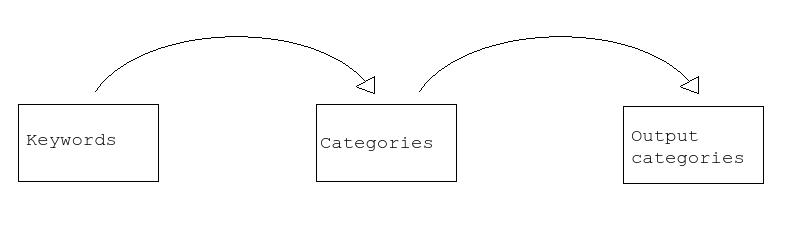
\includegraphics[width=1\textwidth]{classification_process.jpeg}
\caption{The classification process}
\label{fig:classification_process}
\end{figure}
%This classifier will be used as part of an automatic categorization process. 
%Our overall goal is therefore to make an automatic categorization that have a predefined keyword list and start by creating a mapping from each keyword to a category from another predefined list. Where the category of a text can be defined from the keywords found in the text. 

\chapter{Categorization}
The process of grouping collections of text into categories can, as already mentioned, be done by either humans or computers. Computer categorization is part of machine learning and is defined as the technique of teaching the machine how to behave. The process is about finding patterns, for instance recognize similarities between input, or to decide rules for the machine so that is is able to predict the category for an input. The goal for the process is to make the behavior of the machine so optimal as possible. Categorization with machine learning can be split into further types; statistical classification which is a \textit{supervised} learning process, and clustering which can be performed as both an \textit{supervised} and an \textit{unsupervised} learning process. Supervised learning is a technique where the machine is given a training data set, where the set contains the correct output in addition to the input we want to classify. The classifier use this data to learn the machine how to behave, also called training the classifier. Unsupervised learning, on the other hand, is the task of trying to find a hidden structure in unlabeled data. The difference is that unlabeled data gives no feedback to the classifier. 
%the data is unlabeled is no feedback sent to the classifier. 
The classifier will therefore not know if the result is correct, but will continue to classify assuming that the classification performed so far is correct.  

Our main assumption for content analysis is that articles which contains the same keywords also belong to some of the same categories in Wikipedia. This means that we want create a group of these articles so that similar articles are grouped together. Supervised classification requires, as already mentioned, a training set. The training set of our problem can be defined as articles in Wikipedia since they are already connected to a category within Wikipedia. The task is to create the classifier that use  this information and is able to classify all other articles. 

%does not have a training set because it is almost impossible to create a training set representiing such a large data set. We still have, however,  information about the underlying category structure of the articles in Wikipedia. The goal is therefore to use this information to group similar articles together.
%Our problem is not suitable for supervised machine learning. Trying to solve the problem with supervised classification would lead to some problems that are difficult to solve; it is for instance almost impossible to create a training set to represent such a large data set and it is therefore not possible to create a classification model based on the data. The categorization should therefore be done with unsupervised machine learning, for instance clustering.

The formal definition of cluster analysis or clustering is the task of grouping similar elements together.Hence the group or cluster should contain elements that share similarities or that are more similar to each other than to the rest of the elements. %This means that elements within a group are more similar to each other than to the rest of the elements, or that the elements within the group have some similarities that make them stand out from the others. 
Our problem could therefore be defined as a clustering problem, where each cluster or group is the articles which contains some of the same keywords. We want to sort the texts in such a way that texts with similar content are classified to the same cluster and therefore to same category. The problem needs a mapping process so that collections of texts get clustered together within the predefined set of categories. The predefined set of categories will change depending on the purpose of the classification, for instance would advertisement need a different set of categories than categorization of news articles. A proposal to a predefined category set for advertisement is the category set of IAB. 

\chapter{IAB - Interactive Advertising Bureau}
%The machine learning need a predefined set of categories for the clustering. It is already mentioned that Wikipedia has articles stored under categories and that the categories form a tree or graph structure. The problem is that there are too many categories that are not relevant for our categorization.

%The problem is therefore using IAB's categories for the clustering. 

IAB stands for Interactive Advertising Bureau and is a business organization that develops, researches and maintains industry standards for the online advertising industry. The organization works for coalescing and maintaining standards and practices in online advertising. IAB also does research and share knowledge on the advertisement and is responsible and distributing 86 \% of all the online advertisement in the US. \cite{IABabout}

IAB has a predefined set of categories that are made as part of the Quality Assurance Guidelines Taxonomy. The category set is split into two layers also called tiers. The first tier is a general or broad level where the categories are quite general, for instance \textit{Business} or \textit{Food \& Drinks}. The second tier is a deepening level, where the categories are subcategories of a category in the first tier.
Figure \ref{fig:IAB1} and figure \ref{fig:IAB2}
shows the categories of IAB as defined on their web page and is written as a set of categories. The category set from IAB's taxonomy is a well-defined category set to use of our clustering problem.  




% I stedet kan vi bruke Wikipedia-kategoriene for en sjekk for å se om v har kategoriesert rett?
%
\begin{figure}[H]
\centering
%\begin{subfigure}{\textwidth}
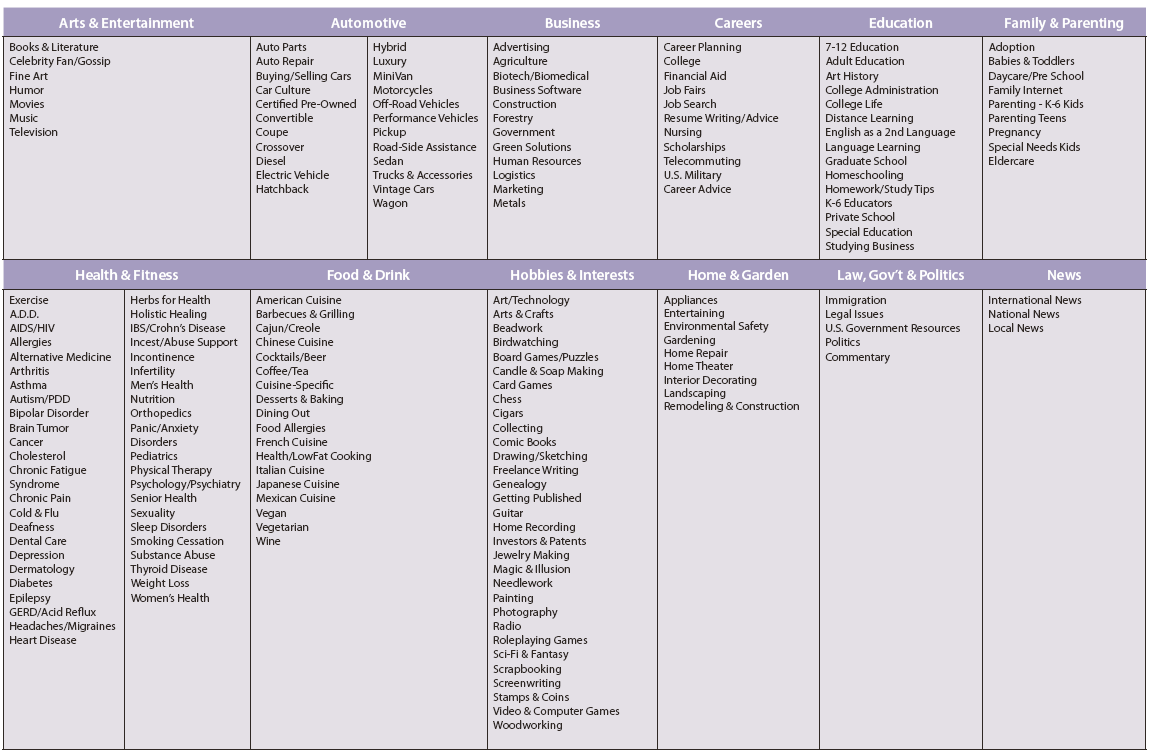
\includegraphics[width=1\textwidth]{IAB/Taxonomy-1.png}
\caption{Categories of the IAB Taxonomy}
\label{fig:IAB1}
\end{figure}
%\end{subfigure}
%\begin{subfigure}{\textwidth}
\begin{figure}[H]
\centering
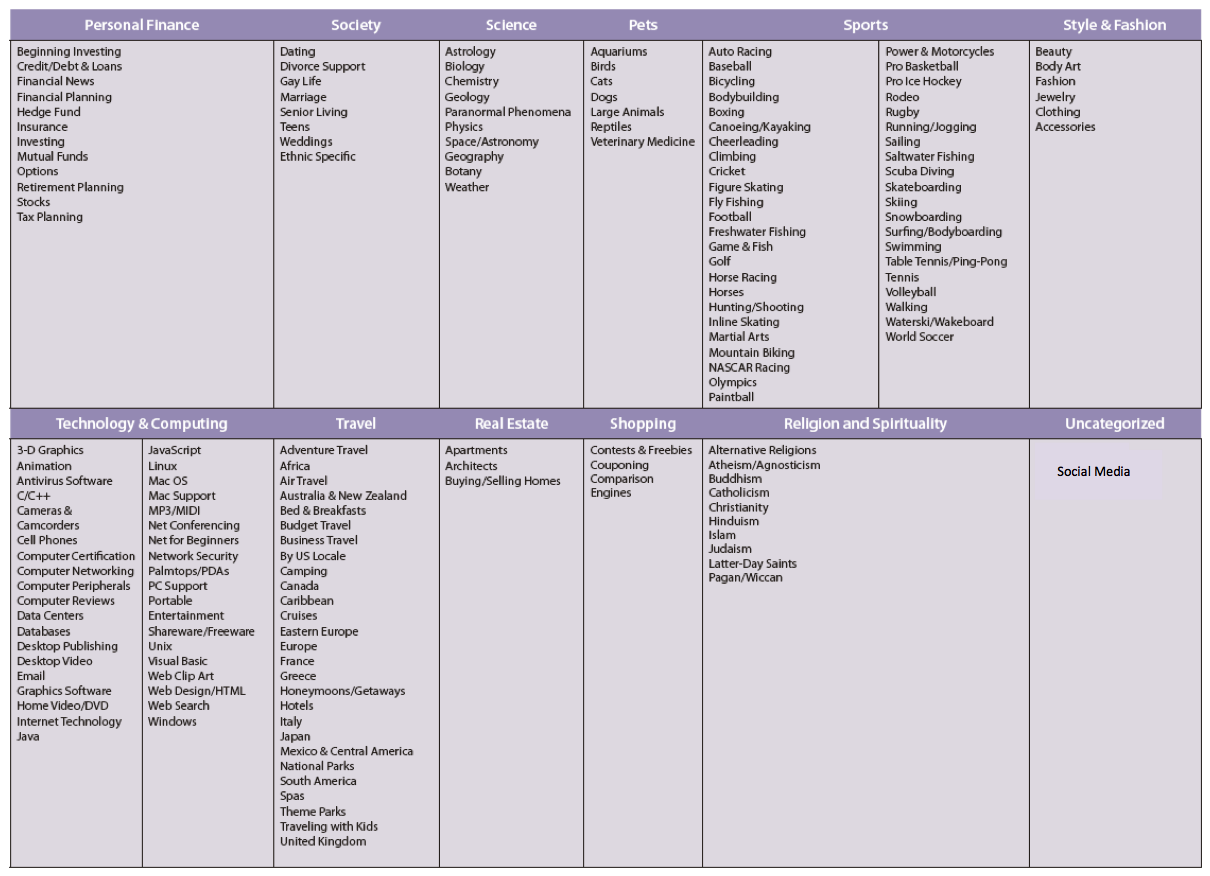
\includegraphics[width=1\textwidth]{IAB/Taxonomy-2.png}
%\end{subfigure}
\caption{Categories of the IAB Taxonomy}
\label{fig:IAB2}
%\label{fig:IAB-categories}
\end{figure}
%Figure \ref{fig:IAB-categories} 


%When categorizing a collection of texts, similar texts will be in the same cluster and therefore in the same category. This can be used to determine the content of the text. 

%The content analysis need a list of keyword to look for in texts. 


\chapter{Wikipedia}
It has already been mentioned that content analysis needs a keyword list for recognizing words or phrases that are useful for classification. We require that the list is so large that it contains almost all the words that give information of possible categories for the content where the keyword is found.  We have chosen to use Wikipedia to create such a keyword list. 

Wikipedia is a free, online encyclopedia and community that was created by Jimmy Wales in 2001. The encyclopedia is edited by the Wiki-principle, which means that everyone can create and edit articles. To understand the importance of Wikipedia it is worth mentioning that the web page has been ranked as the fifth globally most important web page (New York Times, February 2014), with more than  30 million articles and almost 500 unique users a month. 

Wikipedia is ideal to use as a base for the keyword list since it contains lots of articles within many subjects and is maintained by thousands of people. The idea is to base the list on all the titles in Wikipedia, but the list has to be modified to only contain relevant titles. It is for instance not relevant to have common words in the keyword list, like "the" for example, because these will not provide any useful information. It is also important to remove ambiguous words that could confuse the categorization process or apply wrong information. 

There are many advantages of using Wikipedia, one of them is that all articles are already categorized which gives information about a possible category for each category. This means that the process of mapping between keyword and category  easily can be done by the computer. Another advantage is that it contains articles within various fields and is well maintained.

\chapter{Structure of Wikipedia}
The structure of Wikipedia is web based, where articles with similarities are linked together. Since Wikipedia is language-based, articles only link to other articles within the same language. Wikipedia does also have a category structure, where all articles are classified under at least one category. A category could have articles, but could also have subcategories, where the subcategories have their own articles and subcategories. The categories form a large category graph where articles are put under the most describing category, as an example is Ole Johan Dahl \footnote{\olejohandahleng} (Norwegian computer scientist) placed under the category \textit{Norwegian computer scientists} instead of the parent category \textit{Computer scientists by nationality}. 

The category graph is created so there is a link between a category and its subcategories. There is no beginning of the category graph, but here are some categories which have most other categories as their subcategories. These can be though of as beginning categories, often called root categories, and are important when we want to look through all categories in the graph and observe the relationships between them.  Two ategories that can be viewed as potential root categories are \textit{Fundamental Categories} and \textit{Main Topic Classifications}. If one of these are chosen as the root category, we can continue through the graph by looking at its subcategories and proceed by looking at each of the subcategory's subcategories an so on.
%An important 
%The easiest way of looking at all categories in the graph is to choose a root category and follow the links to its subcategories and then continue to look 

Figure \ref{fig: subcat_lindgren} is an example of a structure for the category \textit{Astrid Lindgren}, the swedish children's writer. The figure shows a tree structure for the category from the category graph. The figure shows that the category \textit{Astrid Lindgren} has 7 pages directly under the category, and 3 subcategories: \textit{Astrid Lindgrens karakterer} (7 pages), \textit{Astrid Lindgrens bøker} (9 pages) and \textit{Pippi Langstrømpe} (16 pages).  This means that there are indirectly 39 pages under the category \textit{Astrid Lindgren}. 


%is created and how it is fetched from the page for category information.\footnote{\categorytree}

\begin{figure}[H]
\centering
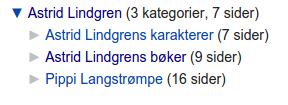
\includegraphics[height=2.5cm]{Dumps/imgs/Kategorier-Astrid-Lindgren.png}
\caption{Subcategories of the category \textit{Astrid Lindgren}. }
\label{fig: subcat_lindgren}
\end{figure}

% HVORFOR IKKE BRUKE WIKIPEDIA SINE KATEGORIER!
Articles of Wikipedia are already classified under categories, but the categorization between articles and categories cannot be used as a pre-defined category set. The reason is that articles in Wikipedia is categorize, but the categories are not guaranteed to be in the pre-defined category set. Hense it is essential that the classifier creates a connection from the article and to a category that is know to exist in the set. The classifier should instead be based on the category information provided by Wikipedia. 

%We will therefore need a mapper to a category we know exists. 
%but we cannot use either the categorization from articles to categories nor 
%this categorization is not ideal. It is not possible to use the categorization since a topic might lead
Another reason why it is not possible to use the category set in Wikipedia as the predefined category set because the category set in Wikipedia is too large. Some categories do not  provide information of the actual content, and some are too specified. There are also cases where articles are categorized under categories where the combination of the categories does not provide any new information. An example is the article of \textit{Ole Johan Dahl}. Some of the article's categories are showed in figure \ref{fig: olejohandahl_categories}. This is an example of an article where the categories provide the same information, i.e., we already know that he was from Norway since he is in the category \textit{People from Mandal, Norway}, so it would be enough to add that he was a computer scientist instead of specifying that he was a Norwegian computer scientist. 

\begin{figure}[H]
\centering
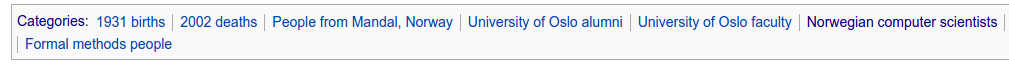
\includegraphics[width=\textwidth]{Dumps/imgs/olejohandahl-categories.png}
\caption{Some categories from the article of Ole Johan Dahl}
\label{fig: olejohandahl_categories}
\end{figure}

%set is not ideal as a predefined category set for our classifier. 
%There are two main reasons why the categories cannot be based on the categories from Wikipedia. 
%A reason for this is that an article in Wikipedia can be categorized under more than one category and these categories might not be the relevant category set. 
%In many cases are the categories directly subcategories of another category, but in some cases could it be a larger path until a common parent category and the category structure would therefore have to be flatten to make sure it is not classified under conflicting categories. 

%Hva tenkte jeg her? Another reason is that Wikipedia contains

\chapter{Domain}
There are many areas where content analysis (the task of understanding the content of the text) is useful, but the two most dominating areas are advertising and improvement of user experience. 
%Content analysis is useful for understanding texts, and is often used in two domains; advertising and improving user experience. 
Advertising is the main income of most online companies that provide free services. The alternative to free services with advertisement is to sell access to to their services, but this is in many cases not possible because the online market is very competitive and many users expect everything on the internet to be free. 

%difficult in many cases because of how competitive the market is and the expectations of a free Internet. 
%Online advertising is a growing market and is the main income of many online companies. 
%Online companies have two ways of earning money, they could either let the user pay to use the services or earn money on advertisement. Most web pages choose the second option because the market is very competitive and many web users expects the web pages to be free. %A newspaper might loose readers when trying to charge them. 

Hence the companies have to earn money without charging the user for their services, and in most cases  this  leads to advertisement. There are different approaches of doing advertisement on web pages. The most common ones are PPC (pay per click) and CPM (cost per mille). CPM is an  advertising technique where the advertiser pays for showing the page to a crowd, while PPC means that an advertisement is shown and the advertiser has to pay for each time a user clicks on the advertisement. Both of the techniques are more valuable for all parts if the advertises are shown to people that are interested and more likely to buy their product. The advertiser has a greater chance of getting customers if the advertisement is shown to the right crowd and the publisher can charge a higher price for the advertisement if the advertiser is more pleased with the result of the advertises.

The main advantage of specified advertisement is that the advertisement can be directed towards users that are more likely to become customers. This means that the advertiser needs to know the users and their interests. Content analysis can be part of building up a profile of the user, since knowing the content of user's text can provide information of the interests of the users. 

\part{Previous Work}
Categorization is not a new topic, neither is taking advantage of Wikipedia in the categorization process. To avoid problems already solved by other projects, has some researching on other projects been done. It has been useful to look at other projects within the same topic and their approaches to solve similar problems. 

\chapter{Classification of tweets}
One of the similar projects is described in the article "Entity Extraction, Linking, Classification, and Tagging for Social Media: A Wikipedia-Based Approach"\cite{entityextraction}. The initial problem is a content analysis problem where they wanted to let the computer understand what the tweets are about and then sort them based on their content. The chosen solution to the problem was to use automatic classification of the tweets, where the tweets were categorized by their content. This problem is very similar to our problem because both the problems are based on understanding texts by recognizing keywords that provide information of categories, i.e., what the tweets are about.

The article describes the categorization as the machine learning process where tweets with similar content are placed in the same class. The authors chose to use Wikipedia as their knowledge base (a repository for information) for finding information of the different categories. The reasons given for why they chose Wikipedia are similar to our reasons;  it is the largest online encyclopedia, it is based on volunteering which means that it is rapidly updated, and it is constantly crawling which is important since it is an advantage to have a fresh, dynamic and timely knowledge base. 

The processing of the tweets required a lot of preprocessing before they could be classified content, especially since tweets are quite sort (max 160 characters).  The preprocessing of the tweets contained several steps before the actual categorization could start, including language detection, cleaning of the tweets (removing everything that is not text), and a tokenizing process (separating sentences into tokens, where a token is defined as a sequence of characters, usually normal words). The described preprocessing is similar to the preprocessing intended for our content analysis because the classifier will only find the keywords if they are an exact match. The classifier depend on tokenizing and cleaning of the words in the text to make them similar to keywords in the keyword list.  

The described tweet classification required some structure to keep information of the tweets and their possible categories. The solution was to create a structure of mentions where a mention is defined on the form ($m_{i}$, $n_{i}$, $s_{i}$), where $m_{i}$ is the string in the tweet we refer to, $n_{i}$ is the node in the knowledge base, and  $s_{i}$ is the< score of the node. All tokens with a connection to the knowledge base (i.e., Wikipedia) were considered relevant, while the others were removed to reduce the complexity. The structure of mentions could be too complex for our case with collections of texts since each text can be much longer than 160 characters, but the idea of keeping track of possible categories is the same. 

A scoring function was used for deciding categories for the tweets, where all the mentions were filtered and some hand-crafted rules were applied. Our project would also need some function to decide what categories are relevant if many categories are proposed. 

\chapter{Evaluation of the classification of tweets}
Evaluation is one of the most important part of a categorization process because it tells if the classification behaves as desired. Classification is, as already mentioned, difficult to evaluate and it was therefore quite useful to look at the evaluation part of the classification of tweets.

The authors argued that the computer classification should be compared by classification done by humans, so that the \textit{predicted} result could be compared with the \textit{correct} result. The problem is that it is very time consuming for humans to classify, so the evaluation was done by sampling 500 tweets. Of these tweets were 477 manually identified by people to give them tags which were compared by the classifier's tags. 

Figure \ref{fig:classification_entities} shows the results of the evaluation phase of the classification. The measures for each tag are P (precision: fraction of retrieved tweets that are relevant), R (recall: fraction of relevant tweets that were tagged) and F1 (F1-score: measure of accuracy, given as $ F_1 = 2 \cdot \frac{\mathrm{precision} \cdot \mathrm{recall}}{\mathrm{precision} + \mathrm{recall}}$). It is interesting to look at the results from the evaluation because they give a good indication on which subjects are difficult to classify. The results show that people and locations are easy to classify, while music is more difficult. This could be because music might contain common words that are dropped from the knowledge base or does not provide useful information while name of locations are easy to recognize for the classifier. 
%One of the most important steps of classifying is the evaluation phase. Evaluation of classifying should be done by humans. Someone will have to look through the results and see how well the classification has been done by comparing the \textit{correct} result with the \textit{predicted} result.

%The article concludes that the tweets that were easiest to classify were about people (see Figure \ref{fig:classification_entities}). This is probably because famous people have their own Wikipedia page, which is easy to match the tweet. The most difficult, on the other hand, was products which seldom have their own page  if the tweet is very specific. 


\begin{figure}[H]
\centering
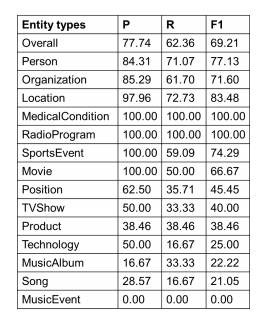
\includegraphics[height=8cm]{Classification_entities}
\caption{The accuracy of the system for extraction and linking.}
%P is the precision, R is the recall and $F_{1}$ is the $F_{1}$-score.} %linking\footnote{\url{http://pages.cs.wisc.edu/~anhai/papers/doctagger-vldb13.pdf, page 8}}}
\label{fig:classification_entities}
\end{figure}


\chapter{Text Categorization with Encyclopedic Knowledge}
The task of making the computer understand the content of text has many difficult challenges that most humans won't encounter. Ambiguous words are for example usually not a problem for humans because it is usually easy to use the context to understand the meaning of the word. Computers on the other hand depend on a dictionary or statics about the word to decide the meaning of the word. Complex sentences could also be a problem for computers, advanced grammar for example can make it difficult to interpret the meaning of the sentence. The paper "Overcoming Brittleness Bottleneck using Wikipedia: Enhancing Text Categorization with Encyclopedic Knowledge"\cite{brittleness}focus on some of these challenges and presents a solution to these. 

One of the main problems in  content analysis performed by a computer is to decide the meaning of a word. Humans have a larger background of knowledge and experience which makes it easier to interpret the meaning of a word. Computers depend on either representing documents as bag of words (BOW) or by learning the context of the word by observation. Context is difficult for a computer because it has to decide the number of words that are needed to decide the context of a word, which obviously depends on the word. 

%Ambiguous words are foten understood from the context, but a computer is then either depending on observing the word in a similar context 

%Ambiguous words or sentences are therefore seldom a  problem for humans because the meaning can be found in the context, but a computer could encounter problems with deciding the meaning if the context is unobserved.

The paper presents a text categorization feature to make it easier for the computer to understand the meaning of a word without analysing the context. A feature is a measure for a property of the observation, for instance is number of occurrences a normal feature for each word in the  BOW. If more than one feature measured for an observation are  usually put together as a feature vector for the observation. The feature generator described in the paper takes text fragments as input and maps these to the most relevant Wikipedia articles. The concepts in the relevant articles are used to find new features, which are added to the augmented bag of words. The authors have chosen the feature generator to be a multi-resolution to generate the best relevant Wikipedia concepts, i.e., it generates features at different levels: individual word level, sentence level, paragraph level and for the whole document. This means that there is a large number of features for each document, and these features are useful to understand the content of the document. 

The feature generator depends on  a text classifier that match documents with the most relevant articles of Wikipedia. The classifier starts by manipulating the text into the same form as the encyclopedic articles. This part resembles our categorization problem since we are also interested in linking texts to Wikipedia or information from Wikipedia.  The discussion about ambiguity is also relevant for our problem, where ambiguous words should either be dropped from the keyword list or the computer will have to find the meaning of the words. 

\chapter{Summary}

\part{General Discussion}

\part{Implementation}
\chapter{Wikipedia's information}
There are two ways of accessing Wikipedia's encyclopedic information. The first way is to look up runtime as most users do when they are looking for information. The other way is more common when the information is used by other programs and

%s, which means that the program access Wikipedia's 

The other, and most common way is to download database dumps from Wikipedia. All Wikipedia articles, images and categories are stored in a database which are accessed when a user are searching for an article online. A database dump is therefore a backup of the database which are usually stored in the case of some data is lost. \footnote{TODO: reference: en.wikipedia.ort/wiki/Database\_dump} This backup is available for anyone interested at \emph{TODO: insert link}\footnote{TODO: insert reference?}. 




A database dump is defined as the table structures which is used to get the information to load

For our purpose there are some dumps that are relevant: 


I have chosen to work on the English Wikipedia, which is the largest database in with *** articles and *** pages. 

The relevant files are: 
\begin{itemize}
\item \enwikicatlink
\item \enwikipage
\item \enwikicategory
\end{itemize}

All of these files are compressed sql-files, which means that they represent files to put information into a SQL-database. Each of the files can be used to build up a database table with insert-statements, so all the information is stored in the table. 

\enwikicatlink describes all the links between categories, which describes two different types of relationships in Wikipedia. The first relationship is between a Wikipedia article and a category, i.e the category *** points to the article. The other relationship is between two categories which means that one of the categories is a subcategory of the other category. 

The file contains the table "categorylinks". Since the file is quite large (1.5GB compressed), it is desirable to split the file into two files; files containing information of the relationships between categories and files that contain information about the relationship between categories and pages. 


\chapter{Parsing through the dumps}
This was solved by creation the program. The program takes the \enwikicatlink as input, and goes through each INSERT-statement in the file. Since all INSERT statements contains information about many relationships, the statements are split to represent one relationship at the time. Then the statement is sorted into "Link between two categories" or "Link between a category and a page" depending on the output of the relationship described in the statement. 

Some of the information about the relationships between categories are not relevant for this problem, for instance information about hidden categories like "Unprinthworthy categories". This categories are removed in the process to reduce the number of category elements considered in the later programs. 

Wikipedia also contains lots of information about redirecting between categories and pages, for instance are article names in plural redirected to the article name in singular.  This information is also stored in \enwikicatlink and is sorted out during the process to be considered later in the process where it is desirable to redirect in the same way, but still not relevant in the early steps of the programming. 

%Category graph builder
One of the output files of the \catlinkprogram is a file containing all relationships between categories. The next step is to sort this information so that a category knows all its subcategories. The program \catgraphbuilderprogram takes the category information as output and creates a structure to represent the information. The output of the program is a file where all parents to a subcategory is stored. %This program should maybe consider loops as well
The program sorts all the categories and output a file where all subcategories of a category is listed under the name of their parent category.

\enwikicatlink also contains some shortcuts for saving space when information about the categories are inserted into the database. An example of such a statement is \footnote{TODO: insert reference: part of the insertion statement from the file \enwikicatlink}: 

\begin{code}
1517681,'fictional_birds','ducks\nfictional ducks','2014-10-26 03:30:11',
'ducks','uppercase','subcat' 
\end{code}

This part of the insertion statements means that the category \emph{fictional ducks} is both a subcategory of the category \emph{Fictional birds} and the category \emph{ducks}. This means that this statement has to result in the following information: 
\begin{code}
Fictional birds: 
* fictional ducks

ducks:
* fictional ducks
\end{code}

One of the problem in the results of the program is that there are potential for loops within the structure. This is because a category may be subcategory of a category, but also the parent category of the same category's parent. This means that the whole structure cannot be represented as a three, but is rather a graph where the connected categories are linked together. 

The other output file of \catlinkprogram is a file where the each line represents an article its immediately closest categories, these categories are the same as those represented at the bottom of the article page. 

It is desirable to get each article's full path for our problem. The next program made is therefore a program that takes creates an output where all articles and their immediate closest categories are stored. Here is also some cleaning done so that all categories which contains the words \emph{Wikipedia} or \emph{category} are removed since these are part of the hidden structure for sorting and not relevant for our task. 

To create the full path of each article are there 

the category graph and all the articles with it's 


%Article builder
After all category links are split into list describing relationships between categories and relationships between articles and their subcategories 



\part{Results and Discussion}

\chapter{Evaluation}
The main purpose of the evaluation is to see whether there are any improvements when applying the categorization, but it is also interesting to evaluate the result of the classifier i.e., see whether it correctly assigns categories. Improvements can also be assumed to be better if the classifier has a high probability of categorize correctly.

%Evaluation of the improvement is an evaluation of the results of the user. 
%The evaluation should both cover evaluation t
%This evaluation can be thought of as two evaluation approaches; evaluation of the technical result and evaluation of the overall improvements when applying the classifier. Technical evaluation is 

%There are different parts of the result that can be evaluated,  but the most important evaluation is to evaluate the classifier to see whether it correctly assign categories. 

The evaluation of the classifier can be separated into different evaluations that together cover the whole categorization. 
%plit into different parts to get an evaluation of the different components of the classifier. 
The first evaluation could be of the predefined base components of the classifier; the keyword list and the set of categories. One way of evaluating the list of keywords is to determine if the keywords are relevant for the categorization. This could be done by looking at the size of the list i.e., how many words are included in the list, and what keywords are actually used (which occur in the collection of text). It could also be interesting to see if some of the words are never used. 

The set of categories could be evaluated as how many texts get categories to the the different categories, and try to evaluate if some of the categories seem unnecessary. The set of categories might also depend on the use of the categorization, which means that some categories might be unnecessary in some content analysis and useful in others. 

A more interesting evaluation is the function that decides what category a keyword maps to. It is not possible to do the mapping by hand since the program is operating with many thousand keywords, also in many languages, which means that the mapping has to be done automatically. The best evaluation of this function is comparing with  a true solution. Creating a true solution for the whole categorization, but there are two other approaches for evaluating the result. The first is to create a handmade solution for some small list and compare the classifier's result with this list. This will hopefully give some indication of the result of the classifier, but the result will vary a lot depending on what list we choose. 
%This should be compared by a list made by humans; what category should a keyword link to? The problem with this is that it is time consuming and difficult to make a list like this by hand. 
The other approach is to take advantage of Wikipedia's category structure. 
%
%of the list could therefore be based on Wikipedia's category structure instead. 
All articles are, as already mentioned, already categorized and it is therefore possible to compare the path 
%Since all titles are categorized is it possible to compare the path 
distances from the parent categories and to the most describing category to determine if the keyword is linking to the right categories.


The last part of the classifier's evaluation is deciding the overall result, i.e., how well does the classifier categorize the collection of texts? The best evaluation would again be to compare the classifier's result with a manual categorization and look if the results are the same. The problem with this approach is the same as with the mapping function, we need a true solution to compare with. A proposal to a result is the same; we could create a small set for comparing, but a problem with this solution is that it is a difficult task for comparing, since text can be difficult to categorize. Ole Johan Dahl could for instance be categorized under both \textit{Norwegian computer scientists} and \textit{computer scientist}, and both of them are correct. Such a comparison would therefore depend on using the same categories which can seem unnatural. It is also possible to compare the result of a classification with classifications of very similar texts to see if the categorization decides the same result. 

Some text collections can also be evaluated with help from the text itself. Lots of news articles are for instance already categorized in the URL, for instance would the URL of an article about sport contain  some information that it is about sport:\texttt{.../sport/...}. A possible solution is therefore to look the URL and see if it matches categories proposed by the classifier. 


\part{Conclusion and Further Work}
\chapter{Summary}
This paper has given a brief introduction to the automatic categorization problem used for content analysis. The main reason for automatic content analysis isthat manual classification is impossible for large collections of text, since it is both time consuming and  depends on experts within the topic of the texts. Automatic content analysis is based on the idea that the computer understands texts by recognizing specific keywords that  connected to one or more predefined categories. The advantages of basing such a keyword list on the titles of articles from Wikipedia is that Wikipedia is a large online encyclopedia that covers lots of subjects and is regularly maintained by lots volunteers. The category set for the classification can vary depending on the purpose of the classification, but it is essential that the predefined set is large enough to cover enough topics, but also so specific that information is preserved. An example of a predefined category set that is well-suited for advertisement is provided by IAB, Interactive Advertising Bureau. 

% often kept up to date. 


%It has discussed the different components needed to perform a content analysis on a collection of texts. Two of the most important components of the classifier has been discussed; a predefined list of keywords where the keywords are based on the titles of Wikipeda, and a predefined set of categories for the result. The paper has also discussed important properties of the predefined category set, followed by other similar work and discussion of evaluation of the classifier, i.e., what parts of the classifier can be evaluated and how this should be done. 

\backmatter{}
\part{References}
\printbibliography

\end{document}
